% --- INICIO DE LA SECCIÓN DE ANEXOS ---

% El comando \appendix cambia la numeración de los capítulos a letras (A, B, C, etc.)
\appendix

% Con \cleardoublepage o \clearpage aseguras que los anexos comiencen en una página nueva.
\cleardoublepage 

% Título principal de la sección de anexos
\chapter*{Anexos}
\addcontentsline{toc}{chapter}{Anexos} % Añade "Anexos" a la tabla de contenido


\chapter{Archivo Docker Compose}
\label{anexo:dockercompose}

\begin{lstlisting}[language=yaml, caption={Contenido del archivo docker-compose.yml para levantar el entorno.}, label={lst:docker-compose}]
services:
  jenkins:
    build: .
    image: ${IMAGE_NAME}
    container_name: ${CONTAINER_NAME}
    restart: always
    ports:
      - "8080:8080"
      - "50000:50000"
    volumes:
      - jenkins_data:/var/jenkins_home
      - /var/run/docker.sock:/var/run/docker.sock
    environment:
      - JENKINS_ADMIN_PASSWORD=${JENKINS_ADMIN_PASSWORD}
      - JAVA_OPTS=${JAVA_OPTS}
      - PIPELINE_NAME=${PIPELINE_NAME}
      - REPO_URL=${REPO_URL}
      - BRANCH=${BRANCH}
      - JENKINSFILE_PATH=${JENKINSFILE_PATH}

volumes:
  jenkins_data:
\end{lstlisting}

\chapter{Archivo Jenkinsfile}
\label{anexo:jenkinsfile}

\begin{lstlisting}[language=groovy, caption={Estructura completa del Jenkinsfile.}, label={lst:jenkinsfile}]
/**
 * =============================================================================
 * PIPELINE DE DEVSECOPS CON ANÁLISIS IA
 * =============================================================================
 * * Este pipeline implementa un ciclo de vida de CI/CD para una aplicación Java,
 * integrando la seguridad como un componente central a través de las siguientes fases:
 * * 1. Compilación y Pruebas Unitarias.
 * 2. Análisis Estático de Seguridad (SAST) con SpotBugs.
 * 3. Análisis Avanzado de Seguridad y Calidad con un modelo de IA.
 * 4. Quality Gate: Detención automática del pipeline si se encuentran vulnerabilidades críticas.
 * 5. Construcción y Despliegue de la aplicación como un contenedor Docker.
 * * =============================================================================
 */
pipeline {
    // Define que el pipeline puede ejecutarse en cualquier agente de Jenkins disponible.
    // Para entornos de producción, se recomienda usar etiquetas para seleccionar agentes específicos.
    agent any

    // --- Variables de Entorno Globales ---
    // Definen parámetros y rutas consistentes a lo largo de todo el pipeline.
    environment {
        // Directorio para almacenar todos los artefactos de análisis generados.
        SCAN_RESULTS_DIR = 'scan-results'
        // Nombre del proyecto, puede usarse para etiquetar artefactos o imágenes.
        PROJECT_NAME = 'demo'
        // Directorio del código fuente a analizar. Se usa una ruta absoluta para mayor robustez.
        JAVA_ANALYSIS_DIR    = "${env.WORKSPACE}/demo/src"
        // Límite de archivos a pasar al script de análisis de IA.
        MAX_FILES_TO_ANALYZE = '10'
    }
    
    // --- Etapas del Pipeline ---
    // Cada 'stage' representa una fase lógica y distinta del proceso de CI/CD.
    stages {

        // Etapa 1: Preparación y Compilación
        // Prepara el entorno, instala dependencias y compila la aplicación.
        stage('Compile & Prepare Environment') {
            steps {
                echo '>>> Stage: Compilando la aplicación y preparando el entorno...'
                
                // Verificación de versiones para diagnóstico.
                sh "java -version"
                sh "python3 --version"

                // Instala las dependencias de Python de forma idempotente.
                sh "pip3 install requests pathlib --break-system-packages || pip3 install requests pathlib || echo 'Dependencies already installed'"
                                
                // Crea el directorio de resultados si no existe.
                sh "mkdir -p ${SCAN_RESULTS_DIR}"
                
                // Entra al directorio del proyecto Java para ejecutar Maven.
                dir('demo') {
                    // Compila y empaqueta la aplicación. 
                    // -Dmaven.test.failure.ignore=true asegura que el pipeline continúe al análisis
                    // de seguridad incluso si las pruebas unitarias fallan, priorizando la seguridad.
                    sh "mvn -Dmaven.test.failure.ignore=true clean package"
                }
            }
        }

        // Etapa 2: Pruebas Unitarias
        // Analiza y publica los resultados de las pruebas unitarias.
        stage('Unit Test Analysis') {
            steps {
                echo '>>> Stage: Publicando resultados de pruebas unitarias...'
                
                // El paso 'junit' parsea los reportes XML y los integra en la UI de Jenkins,
                // mostrando tendencias, fallos y duración de las pruebas.
                junit 'demo/target/surefire-reports/*.xml'
            }
        }
        
        // Etapa 3: Análisis Estático de Seguridad (SAST)
        // Ejecuta herramientas de análisis estático en paralelo para optimizar el tiempo.
        stage('Static Analysis') {
            parallel {
                // Ejecuta SpotBugs para encontrar patrones de error comunes en el código Java.
                stage('SpotBugs SAST') {
                    steps {
                        dir('demo') {
                            script {
                                // El bloque try-catch añade resiliencia. Si SpotBugs falla,
                                // el pipeline no se detendrá, solo se registrará el error.
                                try {
                                    sh "mvn compile spotbugs:spotbugs"
                                    sh "cp target/spotbugsXml.xml ../${SCAN_RESULTS_DIR}/ || echo 'No SpotBugs report found'"
                                } catch (Exception e) {
                                    echo "SpotBugs analysis failed: ${e.getMessage()}"
                                    sh "echo '<BugCollection></BugCollection>' > ../${SCAN_RESULTS_DIR}/spotbugsXml.xml"
                                }
                            }
                        }
                    }
                }
                
                // Recopila los archivos fuente para la siguiente etapa.
                stage('Collect Source Files') {
                    steps {
                        script {
                            sh """
                                find ${JAVA_ANALYSIS_DIR} -name "*.java" -type f > ${SCAN_RESULTS_DIR}/java-files.txt
                                echo "Archivos Java encontrados para análisis:"
                                cat ${SCAN_RESULTS_DIR}/java-files.txt
                            """
                        }
                    }
                }
            }
        }
        
        // Etapa 4: Análisis con Inteligencia Artificial
        // Ejecuta el script de Python personalizado para un análisis de seguridad profundo.
        stage('AI-Powered Analysis') {
            steps {
                script {
                    // Copia el script de análisis al directorio de resultados para aislar la ejecución.
                    sh "cp demo/ai_code_analyzer.py ${SCAN_RESULTS_DIR}/"

                    // Ejecuta los siguientes pasos desde dentro del directorio de resultados.
                    dir(env.SCAN_RESULTS_DIR) {
                        // withCredentials es el mecanismo seguro de Jenkins para manejar secretos.
                        // Inyecta la credencial 'openrouter-api-key' en una variable de entorno
                        // temporal que solo existe dentro de este bloque.
                        withCredentials([string(credentialsId: 'openrouter-api-key', variable: 'OPENROUTER_API_KEY')]) {
                            sh """
                                echo "Iniciando análisis con IA..."
                                python3 ai_code_analyzer.py \\
                                    --directory ${JAVA_ANALYSIS_DIR} \\
                                    --max-files ${MAX_FILES_TO_ANALYZE}
                            """
                        }
                    }
                }
            }
        }    

        // Etapa 5: Quality Gate (Control de Calidad)
        // Punto de control que detiene el pipeline si no se cumplen las políticas de seguridad.
        stage('Quality Gate') {
            steps {
                script {
                    echo '>>> Stage: Verificando políticas de calidad y seguridad...'
                    def resultsFile = "${env.SCAN_RESULTS_DIR}/analysis-results.json"
                    
                    if (fileExists(resultsFile)) {
                        // Lee el archivo JSON generado por el script de IA.
                        def analysisResults = readJSON(file: resultsFile)
                        def highSeverityVulns = analysisResults.summary.high_severity_vulnerabilities
                        
                        echo "-> Vulnerabilidades de severidad ALTA encontradas: ${highSeverityVulns}"
                        
                        // --- Política de Seguridad: Cero Tolerancia para Vulnerabilidades Altas ---
                        if (highSeverityVulns > 0) {
                            // El paso 'error' detiene el pipeline inmediatamente y lo marca como FAILURE.
                            // Esto previene que código inseguro sea construido o desplegado.
                            error("QUALITY GATE FAILED: Se encontraron ${highSeverityVulns} vulnerabilidades de severidad ALTA. Abortando el pipeline.")
                        } else {
                            echo "QUALITY GATE PASSED: No se encontraron vulnerabilidades de severidad ALTA."
                        }
                        
                    } else {
                        // Si el archivo de resultados no existe, es un fallo crítico del proceso de análisis.
                        error("QUALITY GATE FAILED: No se encontró el archivo de resultados '${resultsFile}'. No se puede verificar la calidad.")
                    }
                }
            }
        }

        // Etapa 6: Construcción de Imagen Docker
        // Esta etapa solo se ejecuta si el Quality Gate fue superado.
        stage('Build Docker Image') {
            steps {
                echo '>>> Stage: Construyendo la imagen Docker de la aplicación...'
                script {
                    // El comando 'docker build' usa el Dockerfile de la aplicación.
                    // -f especifica la ruta del Dockerfile.
                    // -t etiqueta la imagen con un nombre y tag (ej: demo-app:latest).
                    // . define el contexto de construcción (el directorio actual).
                    sh 'docker build -f demo/Dockerfile -t demo-app .'
                }
            }
        }

        // Etapa 7: Despliegue en Entorno Local
        // Despliega la imagen construida como un contenedor local.
        stage('Deploy to Local Environment') {
            steps {
                echo '>>> Stage: Desplegando localmente con Docker...'
                
                // Detiene y elimina cualquier contenedor anterior con el mismo nombre.
                // '|| true' evita que el pipeline falle si el contenedor no existe.
                sh 'docker stop demo-app || true'
                sh 'docker rm demo-app || true'

                // Ejecuta el nuevo contenedor.
                // -d: modo detached (en segundo plano).
                // -p 8081:9090 mapea el puerto 9090 del contenedor al 8081 del host.
                // --name asigna un nombre al contenedor para fácil referencia.
                sh 'docker run -d -p 8081:9090 --name demo-app demo-app'
                
                echo '>>> El microservicio debería estar accesible en http://localhost:8081'
            }
        }
    }

    // --- Acciones Post-Ejecución ---
    // Se ejecutan al final del pipeline, sin importar el resultado de las etapas.
    post {
        // 'always' se ejecuta siempre, garantizando que los reportes y artefactos
        // siempre se publiquen, lo cual es crucial para la trazabilidad y el análisis de fallos.
        always {
            echo '>>> Post-execution: Publicando reportes y archivando artefactos...'
            
            // Publica los resultados de JUnit.
            junit(
                allowEmptyResults: true, 
                testResults: 'demo/target/surefire-reports/*.xml'
            )
            
            // Publica el reporte HTML del análisis de IA en la página del build.
            publishHTML([
                allowMissing: false,
                alwaysLinkToLastBuild: true,
                keepAll: true,
                reportDir: env.SCAN_RESULTS_DIR,
                reportFiles: 'ai-analysis-report.html',
                reportName: 'AI Security & Quality Report'
            ])
            
            // Archiva los reportes JSON y HTML como artefactos del build para su descarga.
            archiveArtifacts(
                artifacts: "${env.SCAN_RESULTS_DIR}/*.json, ${env.SCAN_RESULTS_DIR}/*.html",
                allowEmptyArchive: true
            )
        }
        
        // Bloques para notificaciones contextuales (ej. Slack, Email, Teams).
        success {
            echo 'Pipeline completado exitosamente!'
        }
        failure {
            echo 'Pipeline falló! Revisar los logs.'
        }
        unstable {
            echo 'Pipeline completado con advertencias (inestable).'
        }
    }
}
\end{lstlisting}


\chapter{Archivo ai\_analyzer.py}
\label{anexo:ai_analyzer}
\begin{lstlisting}[language=python, caption={Contenido completo del script ai\_analyzer.py.}, label={lst:python_script}]
import json
import os
import requests
import sys
import argparse
from pathlib import Path
from datetime import datetime
import hashlib

class OpenRouterAnalyzer:
    def __init__(self):
        # Leer la API key desde variable de entorno
        self.api_key = os.getenv('OPENROUTER_API_KEY')
        
        # Verificar que la API key esté disponible
        if not self.api_key:
            print("ERROR: La variable de entorno OPENROUTER_API_KEY no está configurada.")
            print("Variables de entorno disponibles:")
            for key, value in os.environ.items():
                if 'OPENROUTER' in key.upper():
                    print(f"  {key}: {value[:10]}...")
            raise ValueError("OPENROUTER_API_KEY no encontrada en las variables de entorno")
        
        print(f"API Key cargada correctamente: {self.api_key[:10]}...")
        
        self.base_url = "https://openrouter.ai/api/v1"
        self.headers = {
            "Authorization": f"Bearer {self.api_key}",
            "Content-Type": "application/json",
            "HTTP-Referer": "http://localhost:8080",
            "X-Title": "Jenkins CI/CD Security Scanner"
        }
        
    def analyze_code_security(self, code_content, filename):
        """Analizar código Java para vulnerabilidades de seguridad"""
        prompt = f"""
Actúa como un experto en seguridad de aplicaciones Java. Analiza el siguiente código fuente para identificar vulnerabilidades de seguridad:

Archivo: {filename}

Busca específicamente:
1. Inyección SQL
2. Cross-Site Scripting (XSS)
3. Problemas de autenticación/autorización
4. Validación de entrada insuficiente
5. Exposición de información sensible
6. Vulnerabilidades de deserialización
7. Uso inseguro de criptografía
8. Path traversal
9. Command injection
10. Problemas de gestión de sesiones

Código a analizar:
```java
{code_content}
```

Responde en formato JSON con la siguiente estructura:
{{
    "vulnerabilities": [
        {{
            "type": "tipo de vulnerabilidad",
            "severity": "HIGH|MEDIUM|LOW",
            "line": "número de línea aproximado",
            "description": "descripción detallada",
            "recommendation": "cómo solucionarlo",
            "code_correction_suggested": "codigo para solucionar la vulnerabilidad",
            "cwe_id": "CWE-XXX si aplica",
            "impact": "impacto potencial de la vulnerabilidad"
        }}
    ],
    "security_score": "puntuación del 0-10",
    "summary": "resumen ejecutivo de los hallazgos"
}}
        """
        
        return self._call_api(prompt, "security")
    
    def analyze_code_quality(self, code_content, filename):
        """Analizar calidad del código Java"""
        prompt = f"""
Actúa como un experto en calidad de código Java. Analiza el siguiente código para identificar problemas de calidad:

Archivo: {filename}

Evalúa:
1. Code smells y anti-patrones
2. Complejidad ciclomática alta
3. Duplicación de código
4. Problemas de mantenibilidad
5. Violaciones de principios SOLID
6. Uso inadecuado de patrones de diseño
7. Gestión de excepciones
8. Nomenclatura y convenciones
9. Eficiencia y rendimiento
10. Cobertura y calidad de comentarios

Código a analizar:
```java
{code_content}
```

Responde en formato JSON:
{{
    "quality_issues": [
        {{
            "type": "tipo de problema",
            "severity": "HIGH|MEDIUM|LOW",
            "line": "número de línea aproximado",
            "description": "descripción del problema",
            "recommendation": "mejora sugerida",
            "code_correction_suggested": "codigo para solucionar el problema",
            "category": "Maintainability|Reliability|Performance|Documentation",
            "effort": "tiempo estimado para solucionar (minutos)"
        }}
    ],
    "quality_score": "puntuación del 0-10",
    "maintainability_index": "índice de mantenibilidad",
    "complexity_score": "puntuación de complejidad",
    "technical_debt": "deuda técnica estimada en minutos"
}}
        """
        
        return self._call_api(prompt, "quality")
    
    def _call_api(self, prompt, analysis_type):
        """Llamar a la API de OpenRouter"""
        payload = {
            "model": "deepseek/deepseek-chat",
            "messages": [
                {
                    "role": "user", 
                    "content": prompt
                }
            ],
            "temperature": 0.1,
            "max_tokens": 4000
        }
        
        try:
            response = requests.post(
                f"{self.base_url}/chat/completions",
                headers=self.headers,
                json=payload,
                timeout=60
            )
            # --- INICIO DE LÍNEAS DE DEPURACIÓN A AGREGAR ---
            print(f"--- DEBUG: Respuesta de la API para '{analysis_type}' ---")
            print(f"Status Code: {response.status_code}")
            print(f"Response Body (Raw): {response.text}")
            print("-------------------------------------------------")
            # --- FIN DE LÍNEAS DE DEPURACIÓN A AGREGAR ---
            if response.status_code == 200:
                result = response.json()
                content = result["choices"][0]["message"]["content"]
                
                # Intentar extraer JSON del contenido
                try:
                    # Buscar JSON en el contenido
                    start = content.find("{")
                    end = content.rfind("}") + 1
                    if start != -1 and end > start:
                        json_content = content[start:end]
                        return json.loads(json_content)
                    else:
                        return {"error": "No se pudo extraer JSON válido", "raw_content": content}
                except json.JSONDecodeError:
                    return {"error": "JSON inválido", "raw_content": content}
            else:
                return {"error": f"API Error: {response.status_code}", "message": response.text}
                
        except Exception as e:
            return {"error": f"Exception: {str(e)}"}
    
    def calculate_overall_score(self, ai_results):
        """Calcular puntuación general del proyecto"""
        total_security_score = 0
        total_quality_score = 0
        valid_files = 0
        
        for result in ai_results.values():
            if isinstance(result, dict) and not result.get('error'):
                if 'security_score' in result:
                    try:
                        total_security_score += float(result['security_score'])
                        valid_files += 1
                    except (ValueError, TypeError):
                        pass
                if 'quality_score' in result:
                    try:
                        total_quality_score += float(result['quality_score'])
                    except (ValueError, TypeError):
                        pass
        
        if valid_files > 0:
            avg_security_score = total_security_score / valid_files
            avg_quality_score = total_quality_score / valid_files
            overall_score = (avg_security_score + avg_quality_score) / 2
            return overall_score, avg_security_score, avg_quality_score
        
        return 0, 0, 0
    
    def generate_report(self, ai_results):
        """Generar reporte HTML comprensivo y moderno"""
        
        # Calcular estadísticas generales
        total_vulnerabilities = sum(len(result.get('vulnerabilities', [])) for result in ai_results.values() if isinstance(result, dict))
        total_quality_issues = sum(len(result.get('quality_issues', [])) for result in ai_results.values() if isinstance(result, dict))
        
        # Contar por severidad
        high_severity_vulns = sum(1 for result in ai_results.values() if isinstance(result, dict) 
                                 for vuln in result.get('vulnerabilities', []) 
                                 if vuln.get('severity') == 'HIGH')
        
        medium_severity_vulns = sum(1 for result in ai_results.values() if isinstance(result, dict) 
                                   for vuln in result.get('vulnerabilities', []) 
                                   if vuln.get('severity') == 'MEDIUM')
        
        low_severity_vulns = sum(1 for result in ai_results.values() if isinstance(result, dict) 
                                for vuln in result.get('vulnerabilities', []) 
                                if vuln.get('severity') == 'LOW')
        
        # Calcular puntuación general
        overall_score, avg_security_score, avg_quality_score = self.calculate_overall_score(ai_results)
        
        # Determinar el estado del quality gate
        quality_gate_status = "PASSED" #if high_severity_vulns == 0 and overall_score >= 7 else "FAILED"
        
        # Generar timestamp
        timestamp = datetime.now().strftime("%Y-%m-%d %H:%M:%S")
        
        html_content = f"""
<!DOCTYPE html>
<html lang="es">
<head>
    <meta charset="UTF-8">
    <meta name="viewport" content="width=device-width, initial-scale=1.0">
    <title>AI Code Analysis Report</title>
    <style>
        * {{
            margin: 0;
            padding: 0;
            box-sizing: border-box;
        }}
        
        body {{
            font-family: -apple-system, BlinkMacSystemFont, 'Segoe UI', Roboto, Oxygen, Ubuntu, Cantarell, sans-serif;
            line-height: 1.6;
            color: #333;
            background: linear-gradient(135deg, #f5f7fa 0%, #c3cfe2 100%);
            min-height: 100vh;
        }}
        
        .container {{
            max-width: 1400px;
            margin: 0 auto;
            padding: 20px;
        }}
        
        .header {{
            background: linear-gradient(135deg, #667eea 0%, #764ba2 100%);
            color: white;
            padding: 30px;
            border-radius: 20px;
            margin-bottom: 30px;
            box-shadow: 0 10px 30px rgba(0,0,0,0.1);
        }}
        
        .header h1 {{
            font-size: 2.5rem;
            margin-bottom: 10px;
            font-weight: 700;
        }}
        
        .header .subtitle {{
            font-size: 1.1rem;
            opacity: 0.9;
            margin-bottom: 20px;
        }}
        
        .meta-info {{
            display: flex;
            gap: 30px;
            font-size: 0.9rem;
            opacity: 0.8;
        }}
        
        .quality-gate {{
            background: {'#d4edda' if quality_gate_status == 'PASSED' else '#f8d7da'};
            color: {'#155724' if quality_gate_status == 'PASSED' else '#721c24'};
            padding: 20px;
            border-radius: 15px;
            margin-bottom: 30px;
            border: 3px solid {'#28a745' if quality_gate_status == 'PASSED' else '#dc3545'};
            text-align: center;
        }}
        
        .quality-gate h2 {{
            font-size: 1.5rem;
            margin-bottom: 10px;
        }}
        
        .metrics-grid {{
            display: grid;
            grid-template-columns: repeat(auto-fit, minmax(250px, 1fr));
            gap: 20px;
            margin-bottom: 30px;
        }}
        
        .metric-card {{
            background: white;
            padding: 25px;
            border-radius: 15px;
            box-shadow: 0 5px 20px rgba(0,0,0,0.08);
            border-left: 5px solid #667eea;
            transition: transform 0.3s ease;
        }}
        
        .metric-card:hover {{
            transform: translateY(-5px);
        }}
        
        .metric-number {{
            font-size: 3rem;
            font-weight: 700;
            margin-bottom: 10px;
        }}
        
        .metric-label {{
            font-size: 0.9rem;
            color: #666;
            text-transform: uppercase;
            letter-spacing: 0.5px;
        }}
        
        .score-card {{
            background: linear-gradient(135deg, #4facfe 0%, #00f2fe 100%);
            color: white;
            border-left: none;
        }}
        
        .severity-high {{ color: #dc3545; }}
        .severity-medium {{ color: #fd7e14; }}
        .severity-low {{ color: #28a745; }}
        
        .files-section {{
            background: white;
            border-radius: 15px;
            padding: 30px;
            margin-bottom: 30px;
            box-shadow: 0 5px 20px rgba(0,0,0,0.08);
        }}
        
        .file-card {{
            background: #f8f9fa;
            border-radius: 10px;
            margin-bottom: 30px;
            overflow: hidden;
            border: 1px solid #e9ecef;
        }}
        
        .file-header {{
            background: linear-gradient(135deg, #667eea 0%, #764ba2 100%);
            color: white;
            padding: 20px;
            font-weight: 600;
        }}
        
        .file-content {{
            padding: 25px;
        }}
        
        .analysis-section {{
            margin-bottom: 30px;
        }}
        
        .section-title {{
            font-size: 1.3rem;
            margin-bottom: 20px;
            color: #333;
            border-bottom: 2px solid #667eea;
            padding-bottom: 10px;
        }}
        
        .issue-card {{
            background: white;
            border-radius: 10px;
            padding: 20px;
            margin-bottom: 15px;
            border-left: 4px solid #667eea;
            box-shadow: 0 2px 10px rgba(0,0,0,0.05);
        }}
        
        .vulnerability-card {{
            border-left-color: #dc3545;
            background: linear-gradient(135deg, #fff5f5 0%, #ffffff 100%);
        }}
        
        .quality-card {{
            border-left-color: #007bff;
            background: linear-gradient(135deg, #f0f8ff 0%, #ffffff 100%);
        }}
        
        .issue-header {{
            display: flex;
            justify-content: space-between;
            align-items: center;
            margin-bottom: 15px;
        }}
        
        .issue-title {{
            font-size: 1.1rem;
            font-weight: 600;
            color: #333;
        }}
        
        .severity-badge {{
            padding: 4px 12px;
            border-radius: 20px;
            font-size: 0.8rem;
            font-weight: 600;
            text-transform: uppercase;
        }}
        
        .severity-high-bg {{
            background: #dc3545;
            color: white;
        }}
        
        .severity-medium-bg {{
            background: #fd7e14;
            color: white;
        }}
        
        .severity-low-bg {{
            background: #28a745;
            color: white;
        }}
        
        .issue-details {{
            display: grid;
            gap: 15px;
        }}
        
        .detail-item {{
            display: flex;
            align-items: flex-start;
            gap: 10px;
        }}
        
        .detail-label {{
            font-weight: 600;
            color: #666;
            min-width: 100px;
        }}
        
        .detail-content {{
            flex: 1;
        }}
        
        .code-block {{
            background: #282c34;
            color: #abb2bf;
            padding: 20px;
            border-radius: 10px;
            overflow-x: auto;
            margin-top: 10px;
            font-family: 'Consolas', 'Monaco', 'Courier New', monospace;
            font-size: 0.9rem;
            line-height: 1.4;
        }}
        
        .code-block pre {{
            margin: 0;
            white-space: pre-wrap;
            word-wrap: break-word;
        }}
        
        .no-issues {{
            text-align: center;
            color: #28a745;
            font-size: 1.1rem;
            padding: 40px;
            background: linear-gradient(135deg, #d4edda 0%, #ffffff 100%);
            border-radius: 10px;
            border: 2px solid #28a745;
        }}
        
        .footer {{
            text-align: center;
            padding: 20px;
            color: #666;
            font-size: 0.9rem;
        }}
        
        @media (max-width: 768px) {{
            .metrics-grid {{
                grid-template-columns: 1fr;
            }}
            
            .header h1 {{
                font-size: 2rem;
            }}
            
            .meta-info {{
                flex-direction: column;
                gap: 10px;
            }}
        }}
    </style>
</head>
<body>
    <div class="container">
        <div class="header">
            <h1>AI Code Analysis Report</h1>
            <div class="subtitle">Análisis inteligente de seguridad y calidad de código</div>
            <div class="meta-info">
                <div>Generado: {timestamp}</div>
                <div>Archivos analizados: {len(ai_results)}</div>
                <div>Powered by AI</div>
            </div>
        </div>
        
        <div class="quality-gate">
            <h2>Quality Gate: {quality_gate_status}</h2>
            <p>{'Tu código cumple con los estándares de calidad' if quality_gate_status == 'PASSED' else 'Se requieren mejoras antes de producción'}</p>
        </div>
        
        <div class="metrics-grid">
            <div class="metric-card score-card">
                <div class="metric-number">{overall_score:.1f}</div>
                <div class="metric-label">Puntuación General</div>
            </div>
            
            <div class="metric-card">
                <div class="metric-number severity-high">{high_severity_vulns}</div>
                <div class="metric-label">Vulnerabilidades Críticas</div>
            </div>
            
            <div class="metric-card">
                <div class="metric-number">{total_vulnerabilities}</div>
                <div class="metric-label">Total Vulnerabilidades</div>
            </div>
            
            <div class="metric-card">
                <div class="metric-number">{total_quality_issues}</div>
                <div class="metric-label">Problemas de Calidad</div>
            </div>
            
            <div class="metric-card">
                <div class="metric-number">{avg_security_score:.1f}</div>
                <div class="metric-label">Puntuación Seguridad</div>
            </div>
            
            <div class="metric-card">
                <div class="metric-number">{avg_quality_score:.1f}</div>
                <div class="metric-label">Puntuación Calidad</div>
            </div>
        </div>
        
        <div class="files-section">
            <h2>Análisis por Archivo</h2>
"""
        
        # Agregar resultados por archivo
        for filename, results in ai_results.items():
            if isinstance(results, dict):
                html_content += f"""
            <div class="file-card">
                <div class="file-header">
                    <div>{filename}</div>
                </div>
                <div class="file-content">
"""
                
                # Análisis de Seguridad
                html_content += """
                    <div class="analysis-section">
                        <h3 class="section-title">Análisis de Seguridad</h3>
"""
                
                vulnerabilities = results.get('vulnerabilities', [])
                if vulnerabilities:
                    for vuln in vulnerabilities:
                        severity = vuln.get('severity', 'LOW')
                        html_content += f"""
                        <div class="issue-card vulnerability-card">
                            <div class="issue-header">
                                <div class="issue-title">{vuln.get('type', 'Unknown Vulnerability')}</div>
                                <div class="severity-badge severity-{severity.lower()}-bg">{severity}</div>
                            </div>
                            <div class="issue-details">
                                <div class="detail-item">
                                    <div class="detail-label">Línea:</div>
                                    <div class="detail-content">{vuln.get('line', 'N/A')}</div>
                                </div>
                                <div class="detail-item">
                                    <div class="detail-label">Descripción:</div>
                                    <div class="detail-content">{vuln.get('description', 'N/A')}</div>
                                </div>
                                <div class="detail-item">
                                    <div class="detail-label">Recomendación:</div>
                                    <div class="detail-content">{vuln.get('recommendation', 'N/A')}</div>
                                </div>
                                <div class="detail-item">
                                    <div class="detail-label">Solución:</div>
                                    <div class="detail-content">
                                        <div class="code-block">
                                            <pre>{vuln.get('code_correction_suggested', 'N/A')}</pre>
                                        </div>
                                    </div>
                                </div>
                            </div>
                        </div>
"""
                else:
                    html_content += """
                        <div class="no-issues">
                            No se encontraron vulnerabilidades de seguridad
                        </div>
"""
                
                html_content += """
                    </div>
"""
                
                # Análisis de Calidad
                html_content += """
                    <div class="analysis-section">
                        <h3 class="section-title">⚡ Análisis de Calidad</h3>
"""
                
                quality_issues = results.get('quality_issues', [])
                if quality_issues:
                    for issue in quality_issues:
                        severity = issue.get('severity', 'LOW')
                        html_content += f"""
                        <div class="issue-card quality-card">
                            <div class="issue-header">
                                <div class="issue-title">{issue.get('type', 'Unknown Issue')}</div>
                                <div class="severity-badge severity-{severity.lower()}-bg">{severity}</div>
                            </div>
                            <div class="issue-details">
                                <div class="detail-item">
                                    <div class="detail-label"> Línea:</div>
                                    <div class="detail-content">{issue.get('line', 'N/A')}</div>
                                </div>
                                <div class="detail-item">
                                    <div class="detail-label">Descripción:</div>
                                    <div class="detail-content">{issue.get('description', 'N/A')}</div>
                                </div>
                                <div class="detail-item">
                                    <div class="detail-label">Recomendación:</div>
                                    <div class="detail-content">{issue.get('recommendation', 'N/A')}</div>
                                </div>
                                <div class="detail-item">
                                    <div class="detail-label">Solución:</div>
                                    <div class="detail-content">
                                        <div class="code-block">
                                            <pre>{issue.get('code_correction_suggested', 'N/A')}</pre>
                                        </div>
                                    </div>
                                </div>
                            </div>
                        </div>
"""
                else:
                    html_content += """
                        <div class="no-issues">
                            No se encontraron problemas significativos de calidad
                        </div>
"""
                
                html_content += """
                    </div>
                </div>
            </div>
"""
        
        html_content += """
        </div>
        
        <div class="footer">
            <p>Reporte generado automáticamente por AI Code Analyzer</p>
            <p>Para más información sobre las vulnerabilidades, consulta OWASP Top 10 y CWE</p>
        </div>
    </div>
</body>
</html>
"""
        
        # Guardar archivo HTML
        with open("ai-analysis-report.html", "w", encoding="utf-8") as f:
            f.write(html_content)
        
        # También generar JSON para quality gates
        report_json = {
            "timestamp": timestamp,
            "overall_score": overall_score,
            "security_score": avg_security_score,
            "quality_score": avg_quality_score,
            "quality_gate_status": quality_gate_status,
            "summary": {
                "total_vulnerabilities": total_vulnerabilities,
                "high_severity_vulnerabilities": high_severity_vulns,
                "medium_severity_vulnerabilities": medium_severity_vulns,
                "low_severity_vulnerabilities": low_severity_vulns,
                "total_quality_issues": total_quality_issues,
                "files_analyzed": len(ai_results)
            },
            "detailed_results": ai_results
        }
        
        with open("analysis-results.json", "w", encoding="utf-8") as f:
            json.dump(report_json, f, indent=2, ensure_ascii=False)

def find_java_files(directory):
    """Buscar archivos Java en un directorio"""
    directory_path = Path(directory)
    
    if not directory_path.exists():
        print(f"El directorio {directory} no existe")
        return []
    
    if not directory_path.is_dir():
        print(f"{directory} no es un directorio válido")
        return []
    
    java_files = list(directory_path.rglob("*.java"))
    print(f"Buscando en: {directory_path.absolute()}")
    print(f"☕ Archivos Java encontrados: {len(java_files)}")
    
    return java_files

def get_analysis_directory():
    """Obtener el directorio a analizar desde argumentos o variables de entorno"""
    
    # Prioridad 1: Argumento de línea de comandos
    parser = argparse.ArgumentParser(description='Analizador de código Java con IA')
    parser.add_argument('--directory', '-d', 
                       help='Directorio a analizar (por defecto: busca en directorio actual)')
    parser.add_argument('--max-files', '-m', type=int, default=5,
                       help='Número máximo de archivos a analizar (por defecto: 5)')
    
    args = parser.parse_args()
    
    # Prioridad 2: Variable de entorno
    env_directory = os.getenv('JAVA_ANALYSIS_DIR')
    
    # Prioridad 3: Directorio por defecto
    if args.directory:
        analysis_dir = args.directory
        print(f"Directorio especificado por argumento: {analysis_dir}")
    elif env_directory:
        analysis_dir = env_directory
        print(f"Directorio especificado por variable de entorno: {analysis_dir}")
    else:
        # Buscar en directorio actual y subdirectorios
        analysis_dir = "."
        print(f"Usando directorio por defecto: {Path('.').absolute()}")
    
    return analysis_dir, args.max_files

def main():
    # Obtener y mostrar el directorio actual
    current_directory = Path.cwd()
    print(f"Directorio actual: {current_directory}")
    
    # Listar archivos en el directorio actual
    print("\nArchivos en el directorio actual:")
    for file in current_directory.iterdir():
        print(f"- {file.name}")
    
    analyzer = OpenRouterAnalyzer()

    # Obtener directorio a analizar
    analysis_directory, max_files = get_analysis_directory()
    
    # Buscar archivos Java
    print(f"\nBuscando archivos Java en: {analysis_directory}")
    java_files = find_java_files(analysis_directory)
    
    if not java_files:
        print(f"No se encontraron archivos Java en {analysis_directory}")
        print("Asegúrate de que el directorio contenga archivos .java")
        
        # Mostrar estructura de directorios para debugging
        analysis_path = Path(analysis_directory)
        if analysis_path.exists():
            print(f"\nEstructura del directorio {analysis_directory}:")
            for item in analysis_path.rglob("*"):
                if item.is_file():
                    print(f"  - {item.relative_to(analysis_path)}")
        
        sys.exit(1)
    
    # Limitar número de archivos a analizar
    files_to_analyze = java_files[:max_files]
    if len(java_files) > max_files:
        print(f"Limitando análisis a {max_files} archivos de {len(java_files)} encontrados")
    
    print(f"\nAnalizando {len(files_to_analyze)} archivos Java con IA...")
    
    ai_results = {}
    
    for java_file in files_to_analyze:
        try:
            with open(java_file, 'r', encoding='utf-8') as f:
                code_content = f.read()
                
            if len(code_content.strip()) == 0:
                continue
                
            print(f"Analizando: {java_file}")
            
            # Análisis de seguridad
            security_result = analyzer.analyze_code_security(code_content, str(java_file))
            
            # Análisis de calidad
            quality_result = analyzer.analyze_code_quality(code_content, str(java_file))
            
            # Combinar resultados
            combined_result = {}
            if isinstance(security_result, dict):
                combined_result.update(security_result)
            if isinstance(quality_result, dict):
                combined_result.update(quality_result)
            
            ai_results[str(java_file)] = combined_result
            
        except Exception as e:
            print(f"Error analizando {java_file}: {e}")
            ai_results[str(java_file)] = {"error": str(e)}
    
    # Generar reporte
    analyzer.generate_report(ai_results)
    
    print("Análisis completado. Reportes generados:")
    print("- ai-analysis-report.html")
    print("- analysis-results.json")

if __name__ == "__main__":
    main()
\end{lstlisting}


\chapter{Reporte de vulnerabilidades mediante IA}
\label{anexo:ai-analysis-report}

% Este comando restaura el estilo de página por defecto (con numeración)
% para la página donde comienza el anexo.
\thispagestyle{plain}

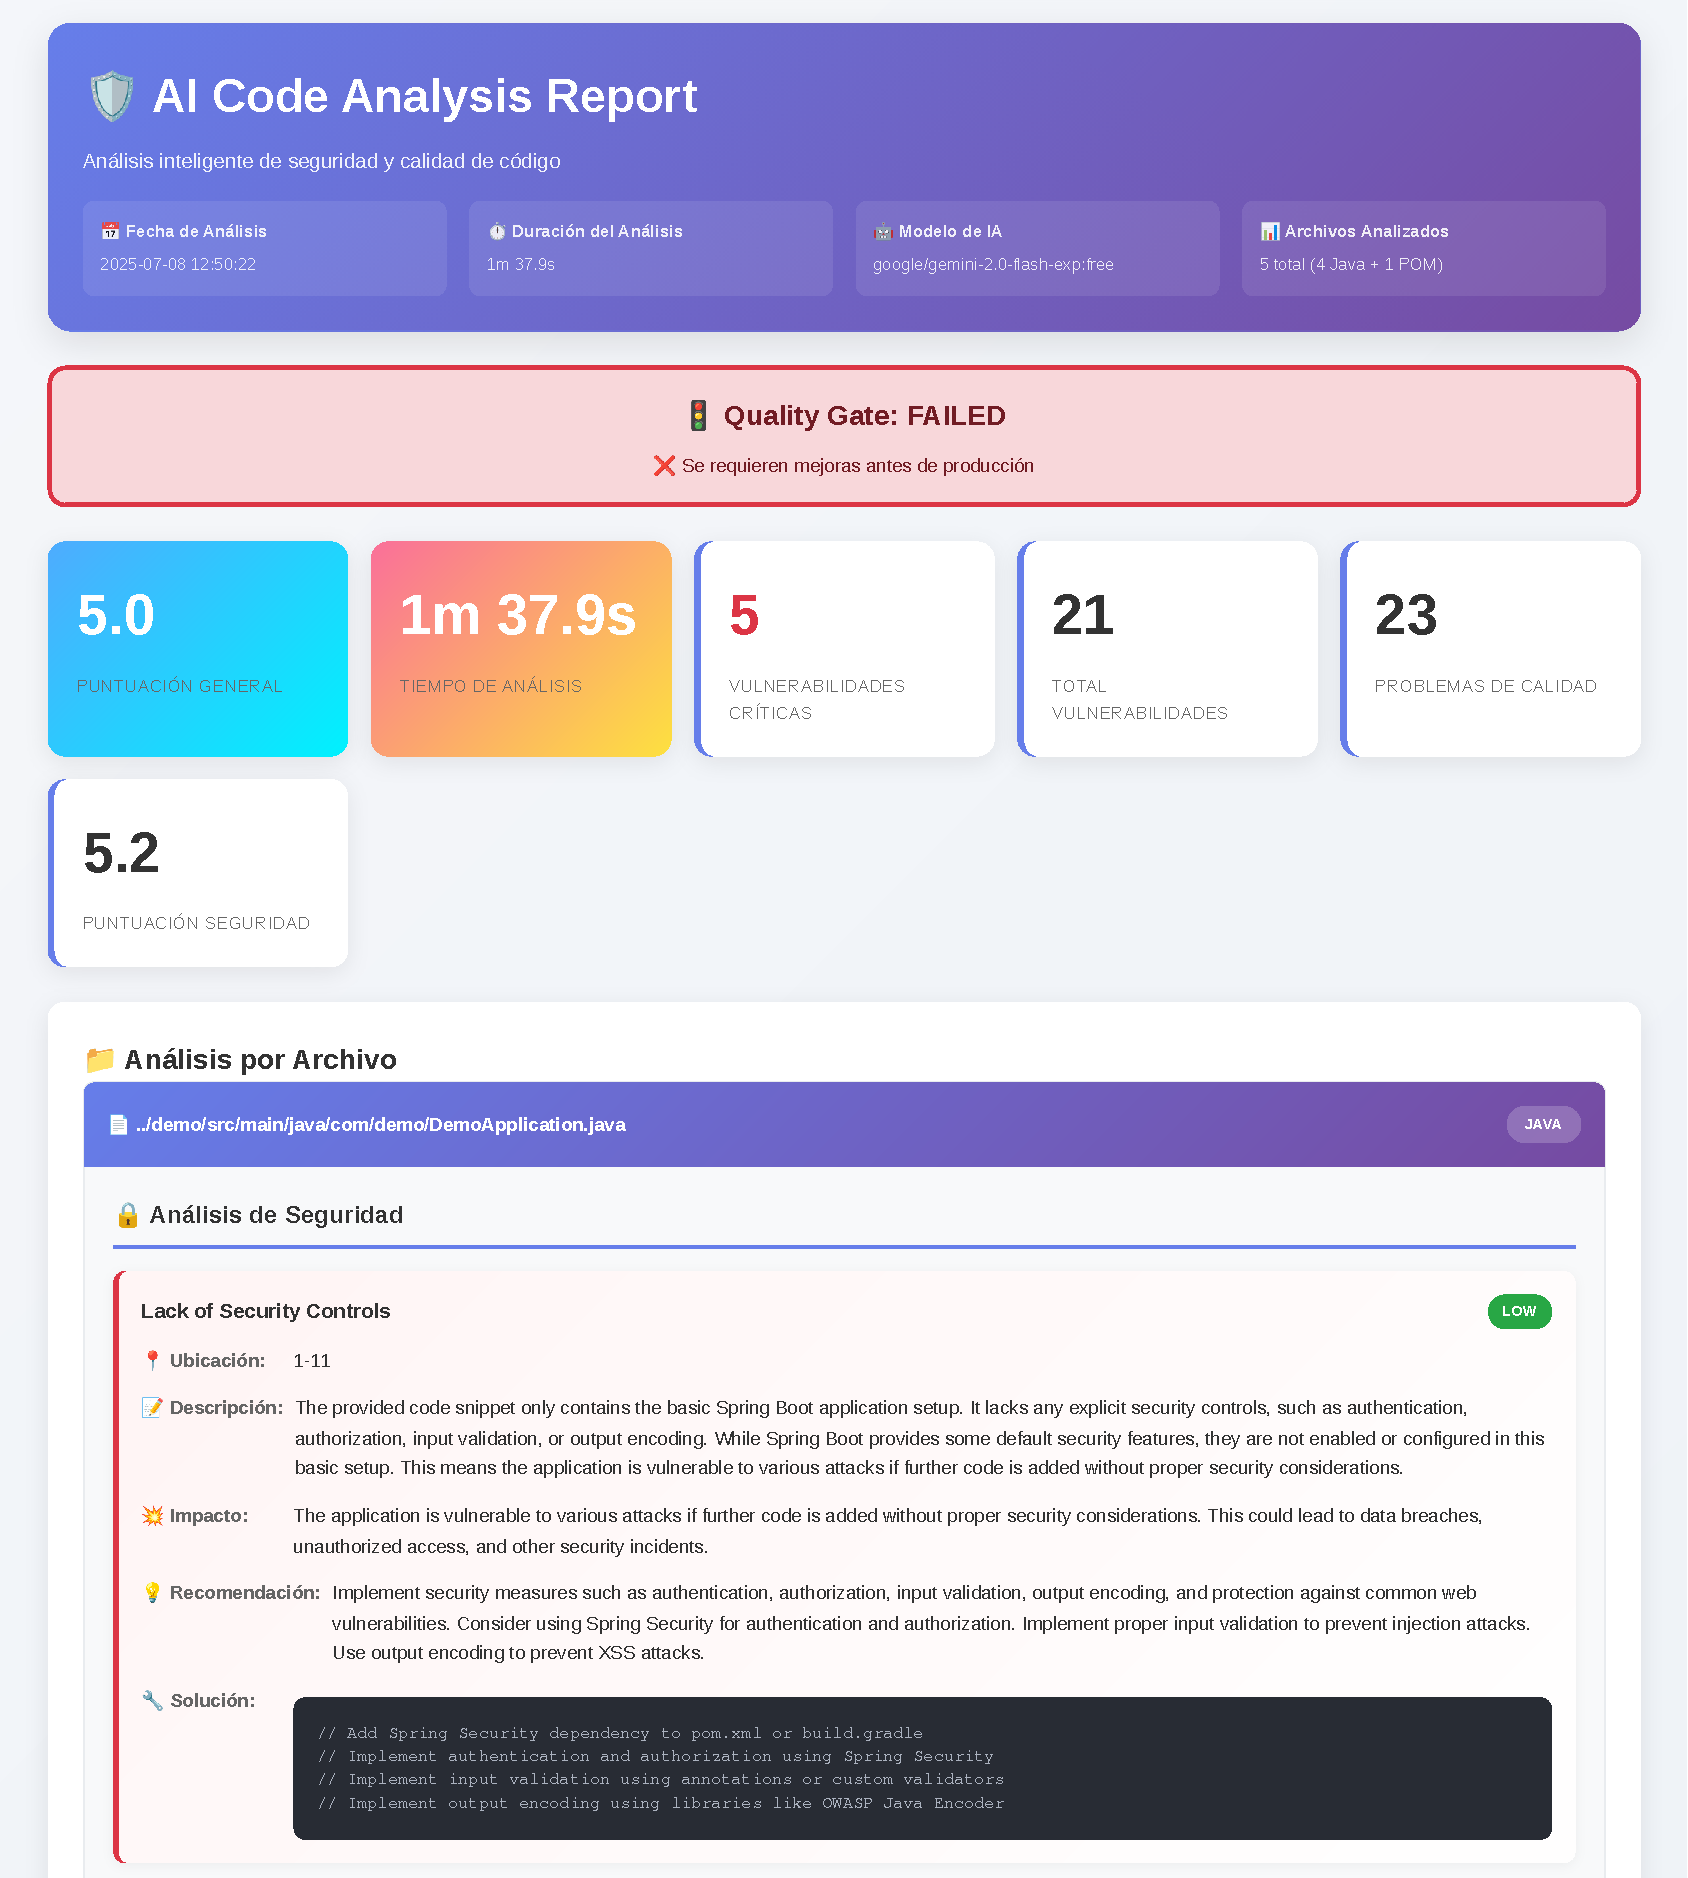
\includepdf[
    pages=-,
    width=\textwidth,
    height=\textheight,
    keepaspectratio,
    % Esta opción aplica el estilo 'plain' (solo número de página)
    % a CADA página del PDF insertado.
    pagecommand={\thispagestyle{plain}}
]{contenido/pdfs/ai-analysis-report.pdf}